 \section{Network Structure}

The network structure \gls{NB-IoT} is very similar to that of legacy \gls{LTE} as can be seen in \autoref{fig:network_structure}. The system is divided into a control plane \gls{CIoT} \gls{EPS} optimization and a user plane \gls{CIoT} \gls{EPS} optimization.

\tikzsetnextfilename{NB-IoT_Network_Architechture}
\begin{figure}[H]
\centering
%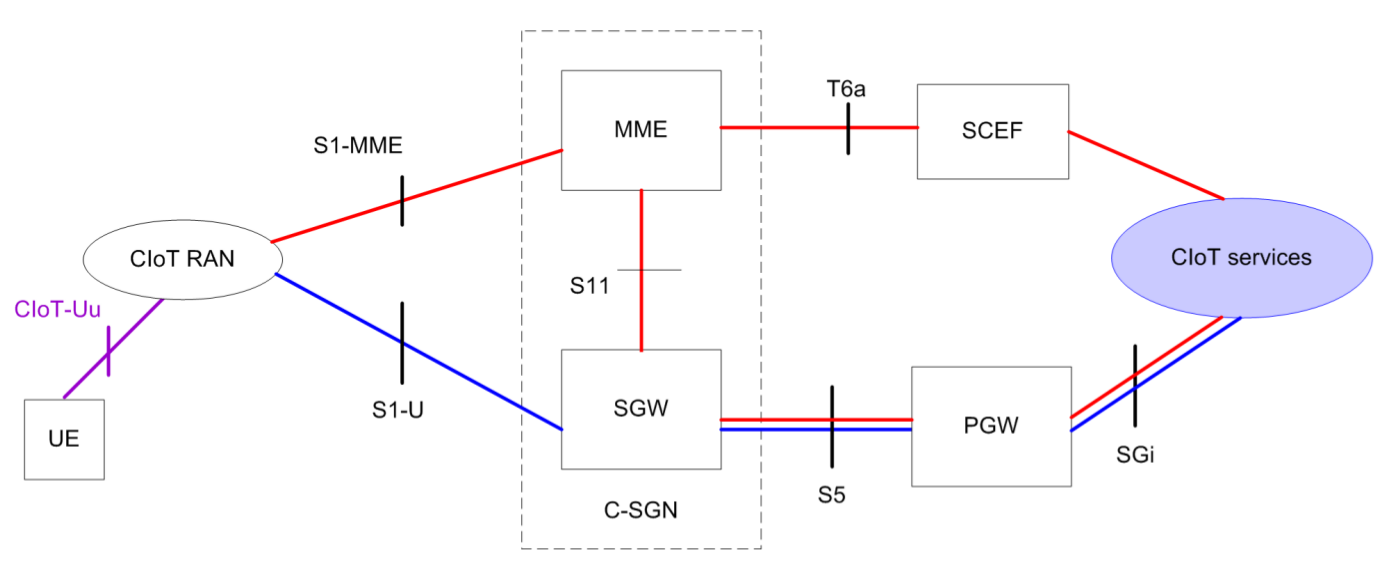
\includegraphics[width=\textwidth]{figures/NB-Network.png}
\definecolor{purple}{HTML}{7030A0}
\usetikzlibrary{arrows}
\definecolor{red}{HTML}{FF0000}
\definecolor{blue}{HTML}{00B0F0}

\resizebox{\textwidth}{!}{
\begin{tikzpicture}[scale=0.5]


\draw  (-14,5) rectangle (-10,3);
\node at (-12,4) {Device};
\draw  (-4,14) rectangle (2,-8);
\draw  (6,9) rectangle (10,7);
\draw  (6,1) rectangle (10,-1);
\node at (-1,-7) {\acrshort{CIoT} \acrshort{RAN}};
\node at (8,8) {\acrshort{MME}};
\node at (8,0) {\acrshort{SGW}};
 




\draw  (14,1) rectangle (18,-1);
\draw  (14,13) rectangle (18,11);
\draw  (25,6) ellipse (3 and 2);
\node at (16,12) {\acrshort{SCEF}};

\node at (16,0) {\acrshort{PGW}};
\node at (25,6) {\acrshort{CIoT} Services};

\draw  (-3,13) rectangle (1,11);
\draw  (-3,5) rectangle (1,3);
\draw  (-3,-3) rectangle (1,-5);
\node at (-1,12) {\acrshort{eNB}};
\node at (-1,4) {\acrshort{eNB}};
\node at (-1,-4) {\acrshort{eNB}};

\draw (6,18) -- (6,15); 
\draw (10,15) -- (10,18);
\draw  (8,18) ellipse (2 and 0.5);
\node at (8,15.4) {\acrshort{HSS}};
\draw (6,15) arc (-120:-60:4);

\draw (14,8.6) -- (14,5.6);
\draw (18,5.6) -- (18,8.6);
\draw  (16,8.6) ellipse (2 and 0.5);
\node at (16,6) {\acrshort{PCRF}};
\draw (14,5.6) arc (-120:-60:4);
\node (v27) at (16,5) {};


\node (v2) at (-7,4) {\acrshort{CIoT}-Uu};
\node (v1) at (-10,4) {};
\node (v3) at (-4,4) {};
\draw [draw=purple, arrows={triangle 45-},fill=purple] (v1) edge (v2);
\draw [draw=purple, arrows={-triangle 45},fill=purple] (v2) edge (v3);

\node (v5) at (-1,8) {X2};
\node (v8) at (-1,0) {X2};
\node (v4) at (-1,11) {};
\node (v6) at (-1,5) {};
\node (v7) at (-1,3) {};
\node (v9) at (-1,-3) {};
\draw [draw=red, arrows={triangle 45-},fill=red] (v4) edge (v5);
\draw [draw=red, arrows={-triangle 45},fill=red] (v5) edge (v6);
\draw [draw=red, arrows={triangle 45-},fill=red] (v7) edge (v8);
\draw [draw=red, arrows={-triangle 45},fill=red] (v8) edge (v9);
\node (v10) at (2,4) {};
\node (v14) at (6,0) {};
\node (v12) at (6,8) {};
\node (v18) at (8,7) {};
\node (v20) at (8,1) {};
\node (v17) at (8,9) {};
\node (v15) at (8,14.4) {};
\node (v21) at (10,8) {};
\node (v23) at (14,12) {};

\node (v24) at (10,0) {};
\node (v26) at (14,0) {};

\node (v33) at (18,0) {};
\node (v32) at (22,6) {};
\node (v30) at (18,12) {};
\node (v29) at (16,1) {};

\node (v11) at (4,6) {S1-\acrshort{MME}};
\node (v13) at (4,2) {S1-U};
\node (v19) at (8,4) {S11};
\node (v16) at (8,12) {S6a};
\node (v22) at (12,10) {T6a};
\node (v25) at (12,0) {S5};
\node (v28) at (16,3) {S7};
%\node (v31) at (20,9) {};
\node (v34) at (20,3) {SGi};

\draw [draw=red, arrows={triangle 45-},fill=red]  (v10) edge (v11);
\draw [draw=red, arrows={-triangle 45},fill=red]  (v11) edge (v12);
\draw [draw=blue, arrows={triangle 45-},fill=blue]  (v10) edge (v13);
\draw [draw=blue, arrows={-triangle 45},fill=blue]  (v13) edge (v14);


\draw [draw=red, arrows={triangle 45-},fill=red]   (v15) edge (v16);
\draw [draw=red, arrows={-triangle 45},fill=red]  (v16) edge (v17);
\draw [draw=red, arrows={triangle 45-},fill=red]  (v18) edge (v19);
\draw [draw=red, arrows={-triangle 45},fill=red]  (v19) edge (v20);
\draw [draw=red, arrows={triangle 45-},fill=red]  (v21) edge (v22);
\draw [draw=red, arrows={-triangle 45},fill=red]  (v22) edge (v23);
\draw [draw=purple, arrows={triangle 45-},fill=purple]  (v24) edge (v25);
\draw [draw=purple, arrows={-triangle 45},fill=purple]  (v25) edge (v26);
\draw [draw=red, arrows={triangle 45-},fill=red]  (v27) edge (v28);
\draw [draw=red, arrows={-triangle 45},fill=red]  (v28) edge (v29);
\draw [draw=red, arrows={triangle 45-triangle 45},fill=red]  (v30) edge (v32);
%\draw [draw=red, arrows={-triangle 45},fill=red]  (v31) edge (v32);
\draw [draw=purple, arrows={triangle 45-},fill=purple]  (v33) edge (v34);
\draw [draw=purple, arrows={-triangle 45},fill=purple]  (v34) edge (v32);
\end{tikzpicture}
}
\caption{Overview over the network blocks and interfaces between blocks in \gls{NB-IoT}. Blue lines are user plane \gls{CIoT} \gls{EPS} optimization, the red lines are control plane \gls{CIoT} \gls{EPS} optimization plane and the purple lines are both \citep{NB_slide}}
\label{fig:network_structure}
\end{figure}


\textbf{\gls{UE}}\\
The \gls{UE} is the smart meters or other products as mentioned, they do not need to transmit a lot of data and it is not critical that it arrives within a certain time frame. They do however require a long battery life time. The problem comes in terms of placement, because many of these devices might be placed in basement like environment which means an increased path loss. The system needs to be able to operate with a \gls{MCL} of 164 dB \citep{REL-13}. As in previous systems the \gls{USIM} is located on the \gls{UE} for authentication purpose \citep[ch. 3]{book_LTE_for_UMTS}.

\textbf{\gls{CIoT} \gls{RAN}}\\
The \gls{CIoT} \gls{RAN} is the base stations, the most typically used is the \gls{eNB} base station. All radio communication terminates at this node. Any \gls{UE} that wish to use an external service, interfaces with the \gls{eNB} \citep{book_LTE_for_UMTS}. The \gls{eNB} interfaces with both the \gls{MME} and the \gls{SGW}. On the control plane (connection to the \gls{MME}) the \gls{eNB} is in charge of \gls{RRM}, i.e. allocating radio resources in the user plane to the individual \gls{UE} based on \gls{QoS} measures. 

\textbf{\gls{MME}}\\
The \gls{MME} takes care of mobility issues, it also keep track of where in the network different \gls{UE}s are connected \citepalias{3GPP_MME_spec}. Another very important function of the \gls{MME} is to handle authentication of \gls{UE}s and setting up security for the data bearers. The \gls{MME} might be connected to multiple \gls{UE}s, however a \gls{UE} may only be connected to a single \gls{MME} \citep[ch. 3]{book_LTE_for_UMTS}. In \gls{NB-IoT} handovers are omitted and the only way to change cell is by releasing the existing connection \citep{REL-13}. The \gls{MME} also handles paging procedures \citep{NB-IoT_Book}.

\textbf{\gls{HSS}}\\
The \gls{HSS} stores the identity of the users, which the \gls{MME} uses for authentication purposes. It records the location of the \gls{UE} in level of visited network control nodes  such as \gls{MME}, it also keep track of which networks the user is allowed to roam to \citep[ch. 3]{book_LTE_for_UMTS}.

\textbf{\gls{SCEF}}\\
The \gls{SCEF} is a multi functional unit, task it handles include: device trigger delivery, sponsored data, \gls{UE} reachability, \gls{3GPP} network issues, \gls{QoS} for a \gls{UE} session etc. Many of these functionalities are meant for normal \gls{LTE} use. Uses meant for \gls{NB-IoT} include \gls{UE} reachability which enables the application layer to be informed when a \gls{UE} reconnects to the network i.e. after an \gls{eDRX} or after \gls{PSM}. Another functionality it handles is \gls{NIDD}, which enables \gls{UE}s with small data volumes to send it data with less overhead and thereby have a longer battery life time \citepalias{3GPP_SCEF_primer}.

\textbf{\gls{SGW}}\\
The \gls{SGW} is primarily a routing unit. It interfaces with the \gls{eNB}, the \gls{MME} and the \gls{PGW}. When the \gls{UE} transmit data it is send to the \gls{eNB} and then routed via the \gls{SGW} to the \gls{PGW} before reaching the providers. The \gls{SGW} typically serve a particular geographic area with several \gls{eNB}s, likewise could the \gls{MME} also serve a particular geographic area. In \gls{LTE} this was the last node in the network that could change during a connected state meaning that all \gls{SGW}s needs to be connected to all \gls{PGW}s \citep[ch. 3]{book_LTE_for_UMTS}. This is however not equally important in \gls{NB-IoT} as no handovers are expected \citep{REL-13}. During connected state the \gls{SGW} works as a relay, however in idle mode the resources are released in the \gls{eNB} and the data path terminates at the \gls{SGW} it then stores the data from the \gls{PGW} and request the \gls{MME} to initiate paging of the \gls{UE} \citep[ch. 3]{book_LTE_for_UMTS}.

\textbf{\gls{PGW}}\\
The \gls{PGW} is the edge of the \gls{EPS}. It function as the point of attachment for the \gls{UE}s \gls{IP} traffic. The \gls{IP}-address of the \gls{UE} is allocated during the connection procedure when the \gls{UE} request a \gls{PDN} connection and during any subsequent \gls{PDN} connection request. It is the \gls{PGW} that performs the \gls{DHCP} functionality \citep[ch. 3]{book_LTE_for_UMTS}. The \gls{PGW} handle interfaces to external CIoT services on a higher level.

\textbf{\gls{PCRF}}\\
The \gls{PCRF} is a server that makes decision on how to handle services provided for the \gls{UE} in terms of \gls{QoS}. It informs the \gls{PGW} and if applicable the \gls{SGW} about appropriate bearer policy can be set up. A default bearer is set up during connection request and either the \gls{UE} or the service domain can request additional bearers which is handled by the \gls{PCRF} \citep[ch. 3]{book_LTE_for_UMTS}.

\textbf{\gls{CIoT} services}\\
The \gls{CIoT} services are typically storage functionalities, but could be control algorithms or other services needed for specific products. 

%connections across the network